% todo : change the image sizes and include again


\documentclass[a4paper]{article}
\usepackage{url}
  \let\oldurl\url
\usepackage{hyperref}
  \let\linkurl\url
  \let\url\oldurl
\usepackage[english]{babel}
\usepackage[utf8]{inputenc}
\usepackage{amsmath}
\usepackage{graphicx}
\usepackage[colorinlistoftodos]{todonotes}
\usepackage{float}


\usepackage{listings}
\usepackage{color} %red, green, blue, yellow, cyan, magenta, black, white
\definecolor{mygreen}{RGB}{28,172,0} % color values Red, Green, Blue
\definecolor{mylilas}{RGB}{170,55,241}

% For citations
\usepackage{natbib}
\setcitestyle{authoryear,round,citesep={;},aysep={,},yysep={;}}

\title{Title}

\author{Shanjit S. Jajmann}

\date{\today}

\begin{document}

%Code Highlight
\lstset{language=C++,%
    %basicstyle=\color{red},
    breaklines=true,%
    morekeywords={matlab2tikz},
    keywordstyle=\color{blue},%
    morekeywords=[2]{1}, keywordstyle=[2]{\color{black}},
    identifierstyle=\color{black},%
    stringstyle=\color{mylilas},
    commentstyle=\color{mygreen},%
    showstringspaces=false,%without this there will be a symbol in the places where there is a space
    numbers=left,%
    numberstyle={\tiny \color{black}},% size of the numbers
    numbersep=9pt, % this defines how far the numbers are from the text
    emph=[1]{for,end,break},emphstyle=[1]\color{red}, %some words to emphasise
    %emph=[2]{word1,word2}, emphstyle=[2]{style},    
}


\maketitle

\section*{Section 1}

\cite{Samuel59}, \cite{mitchell80}

\begin{figure}[H]
\centerline{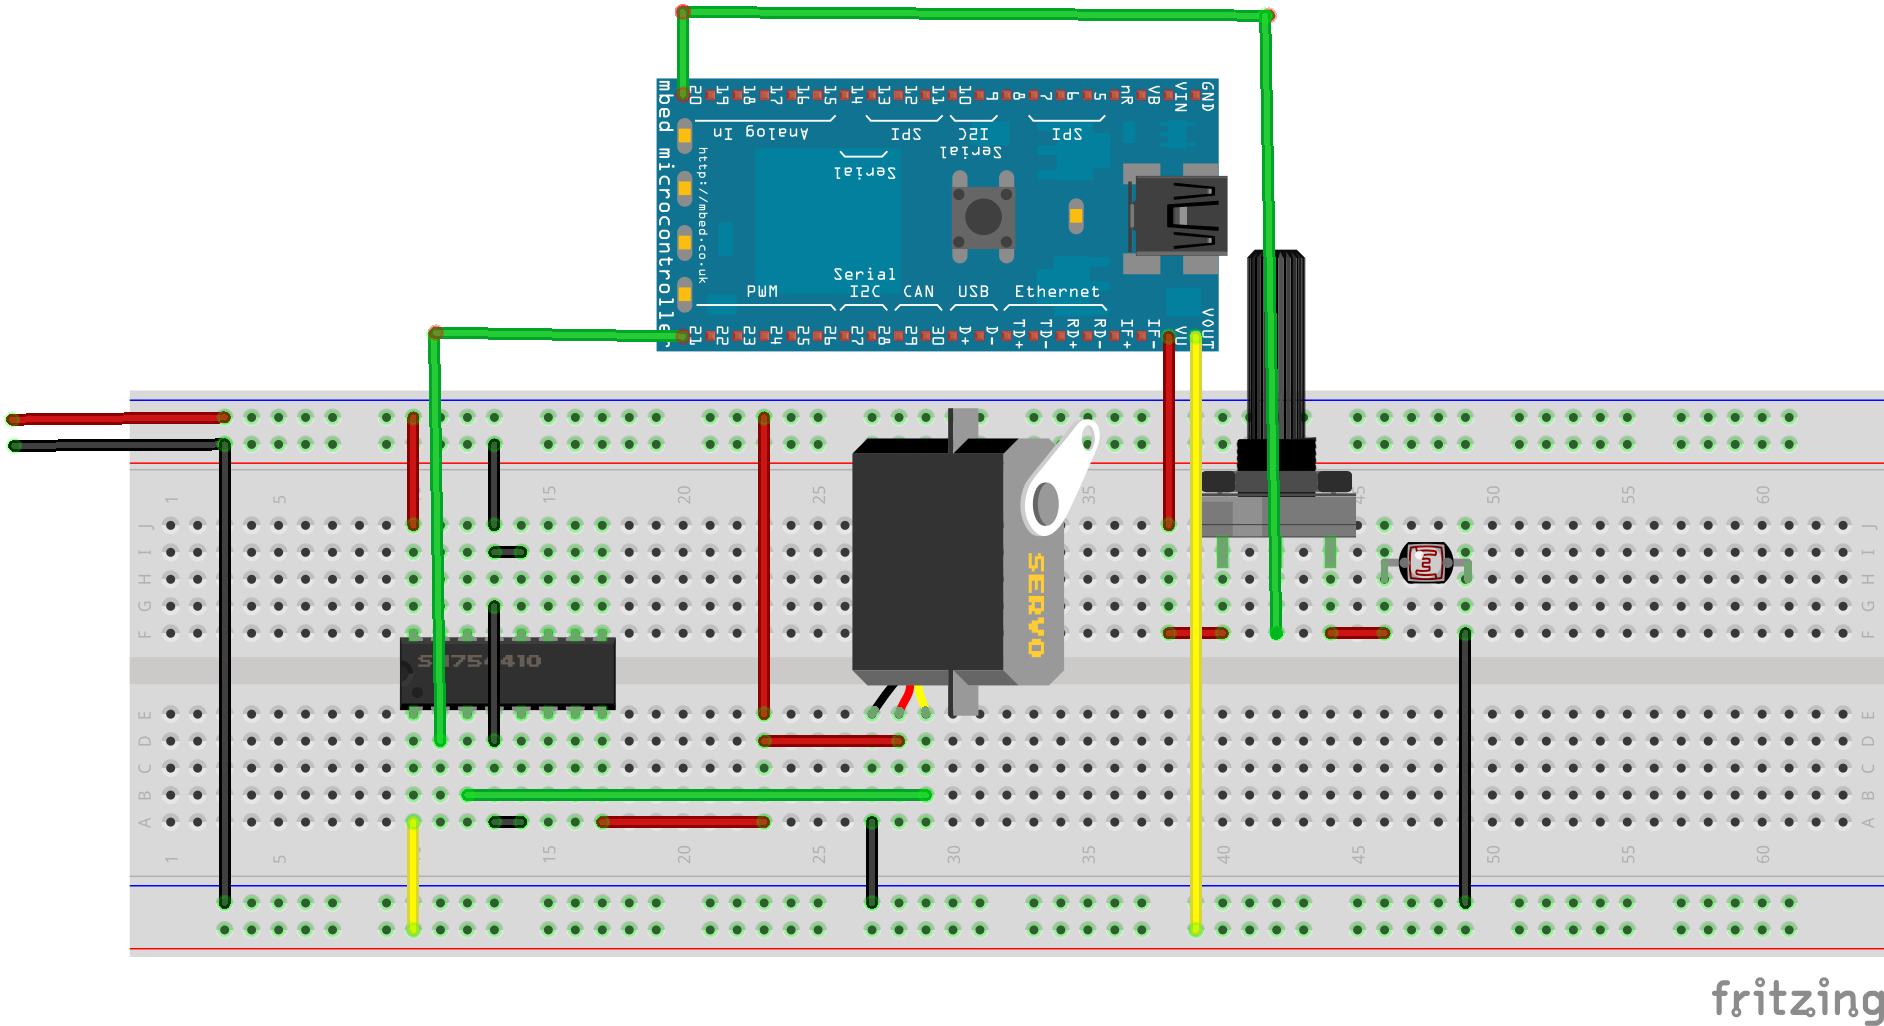
\includegraphics[width=10cm, height=7cm]{fritzing.png}}
\caption{\label{fig:hw}Hardware Connections}
\end{figure}


\section*{Acknowledgments} 
 Acknowledge the awesome people you worked with or under or for. 
 
\bibliography{report}

\bibliographystyle{icml2014}


\end{document}
